% Befehl \fibelkwentry: Ein Eintrag für das Kreuzworträtsel. Vgl. auch Artikel
% „Persoenlichkeitsentwicklung.tex“.
%	Parameter #1: Nummer
%	Parameter #2: Hinweis
\newcommand{\fibelkwentry}[2]{
	% Text um die Breite der Nummerierung einrücken
	\settowidth{\hangindent}{000~}
	% Verhindern, dass innherhalb eines Absatzes auf eine neue Spalte oder
	% Seite umgebrochen wird
	\interlinepenalty=10000
	\makebox[\widthof{000~}][r]{#1~}\ignorespaces#2%
}

\section[Kreuzworträtsel]{}
% brauchen mehr Platz auf der Seite
\enlargethispage{10pt}
\vspace{-1.8cm}
\begin{multicols*}{3}
{% Kein Abstand zw. Paragraphen; linksbündig; kleine Schriftgröße
\parskip=0cm
\RaggedRight
\small

\fibelkwentry{1}{Form des wissenschaftlichen Unterrichts an Hochschulen}

\fibelkwentry{2}{Gegenteil von "fern"}

\fibelkwentry{3}{chem.\ Symbol: Gallium}

\fibelkwentry{4}{Fragewort}

\fibelkwentry{5}{Aufzeichnung hist.\ Ereignisse}

\fibelkwentry{6}{Autor von "Per Anhalter durch die Galaxis"}

\fibelkwentry{7}{Maßeinheit für die Temperatur}

\fibelkwentry{8}{französischer Artikel (f.)}

\fibelkwentry{9}{Abk.: Allgemeiner Studierendenausschuss}

\fibelkwentry{10}{Gebäude des Studierendensekretariats}

\fibelkwentry{11}{Monat}

\fibelkwentry{12}{Maßeinheit für die Zeit}

\fibelkwentry{13}{schnell}

\fibelkwentry{14}{Medium des Lichts?}

\fibelkwentry{15}{Europäische Gemeinschaft}

\fibelkwentry{16}{Heimatuni: \_\_\_\_ Mater}

\fibelkwentry{17}{Segelfliegen: Luftströmung}

\fibelkwentry{18}{Erregung}

\fibelkwentry{19}{nicht Mikro, sondern\dots}

\fibelkwentry{20}{lat.: ich}

\fibelkwentry{21}{engl.: wählen (Telefon)}

\fibelkwentry{22}{erleuchten}

\fibelkwentry{23}{Hersteller von Videospielen}

\fibelkwentry{24}{Zeitmessgerät}

\fibelkwentry{25}{König, Kaiser}

\fibelkwentry{26}{veraltete Einheit des Drucks}

\fibelkwentry{27}{Geburtsland Marie Curies (Abk.)}

\fibelkwentry{28}{bayr.\ Fluss}

\fibelkwentry{29}{Heiligenbild}

\fibelkwentry{30}{16. griech. Buchstabe}

\fibelkwentry{31}{Abk.: Papierchromatographie}

\fibelkwentry{32}{"ohne inneren Antrieb"}

\fibelkwentry{33}{Einheit für Widerstände}

\fibelkwentry{34}{chem.\ Symbol: Zirkonium}

\fibelkwentry{35}{Quotient aus Kraft und Fläche}

\fibelkwentry{36}{nicht angegeben}

\fibelkwentry{37}{Beate \dots}

\fibelkwentry{38}{Abk.: Exponentialfunktion}

\fibelkwentry{39}{Kellner}

\fibelkwentry{40}{Gemälde, Zeichnung, etc.}

\fibelkwentry{41}{Masseneinheit}

\fibelkwentry{42}{nichts Neues, nur \dots}

\fibelkwentry{43}{14. griech. Buchstabe}

\fibelkwentry{44}{Staat in Vorderasien}

\fibelkwentry{45}{feuchter Schnee}

\fibelkwentry{46}{Kurzname für Ulrich}

\fibelkwentry{47}{senkrecht auf einer Ebene stehende Gerade}

\fibelkwentry{48}{geschlossen}

\fibelkwentry{49}{chem.\ Symbol: Lithium}

\fibelkwentry{50}{Beginn des Sommersemesters}

\fibelkwentry{51}{Strahlung der Wärmebildkamera (Abk.)}

\fibelkwentry{52}{Pointe, Glanzpunkt}

\fibelkwentry{53}{dort}

\fibelkwentry{54}{Wertpapier}

\fibelkwentry{55}{Sprengstoff Trinitrotoluol}

\fibelkwentry{56}{griech.: Fertigkeit}

\fibelkwentry{57}{öffentlich-rechtlicher Sender}

\fibelkwentry{58}{erfolgreicher Song}

\fibelkwentry{59}{Mühlenabfall von Getreide}

\fibelkwentry{60}{Abk.: Arbeitskreis}

\fibelkwentry{61}{griech. Vorsilbe: Stern}

\fibelkwentry{62}{lat.\ Vorsilbe: weg-, ent-}

\fibelkwentry{63}{Frau von Fußballer Bastian}

\fibelkwentry{64}{Zahl}

\fibelkwentry{65}{Lehre von den Eigenschaften bewegter Flüssigkeiten}

\fibelkwentry{66}{Abk.: Institutsgruppe}

\fibelkwentry{67}{Abk.: Innenministerium}

\fibelkwentry{68}{Freundlichkeit}

\fibelkwentry{69}{unverschmutzt}

\fibelkwentry{70}{Abk.: erneuerbare Energien}

\fibelkwentry{71}{Thermodynamik: "Linien mit konstantem Volumen"}

\fibelkwentry{72}{englischer Kuchen}

\fibelkwentry{73}{engl.: Ende}

\fibelkwentry{74}{musikalisches Muster}

\fibelkwentry{75}{chem.\ Symbol: Helium}

\fibelkwentry{76}{Menschenmenge}

\fibelkwentry{77}{Europäische Weltraumorganisation}

\fibelkwentry{78}{frz.: hören}

\fibelkwentry{79}{kurze Prüfung z.B. im Praktikum}

\fibelkwentry{80}{Dreiländer\dots}

\fibelkwentry{81}{weibl. Vorname: \_\_\_ Basinger}

\fibelkwentry{82}{Maßeinheit für eine Datenmenge}

\fibelkwentry{83}{Schauspieler: Robert\dots}

\fibelkwentry{84}{moralisch}

\fibelkwentry{85}{viele; große Anzahl}

\fibelkwentry{86}{Zeit, in der die Hälfte der Atomkerne zerfällt}

\fibelkwentry{87}{Abk.: Knockout}

\fibelkwentry{88}{Mannschaft}

\fibelkwentry{89}{Onomatopoetikum des Lachens}

\fibelkwentry{90}{Bewegung des Fußes}

\fibelkwentry{91}{Ampelfarbe, die Radfahrer oft ignorieren}

\fibelkwentry{92}{Adresse eines Computers}

\fibelkwentry{93}{mit zwei Aspekten, doppelt}

\fibelkwentry{94}{Konjunktionswort}

\fibelkwentry{95}{römischer Sonnengott}

\fibelkwentry{96}{Abk.: "center for soft nanoscience"}

\fibelkwentry{97}{Großvater}

\fibelkwentry{98}{veraltete Einheit der Kraft}

\fibelkwentry{99}{frz.: Anfang}

\fibelkwentry{100}{Abk.: InterCity}

\fibelkwentry{101}{Gesangsgruppe}

\fibelkwentry{102}{geflochtener Behälter}

\fibelkwentry{103}{Außerirdisches Wesen}

\fibelkwentry{104}{gerichtete Zukunftsprognose}

\fibelkwentry{105}{22. griech. Buchstabe}

\fibelkwentry{106}{Horrorroman von Stephen King}

\fibelkwentry{107}{engl.: alt/neu}

\fibelkwentry{108}{Abk.: Technische Hochschule}

\fibelkwentry{109}{Abk.: Bachelor}

\fibelkwentry{110}{aus vielen Lichtquanten erstelltes Abbild}

\fibelkwentry{111}{Kapitän der Enterprise}

\fibelkwentry{112}{ein Edelgas (Abk.)}

\fibelkwentry{113}{"Besserwisser"}

\fibelkwentry{114}{Durcheinander}

\fibelkwentry{115}{Einheit: "Lichtjahr"}

\fibelkwentry{116}{griech. Vorsilbe: Luft}

\fibelkwentry{117}{französischer Artikel (m.)}

\fibelkwentry{118}{Zustimmungswort}

\fibelkwentry{119}{"Studentenrestaurant"}

\fibelkwentry{120}{Kfz-Zeichen für Münster}

\fibelkwentry{121}{lat.\ Vorsilbe: zu-, hin-, an-}

\fibelkwentry{122}{sich im Rhythmus bewegen}

\fibelkwentry{123}{Autokennzeichen für Steinfurt}

\fibelkwentry{124}{Wildkatze}

\fibelkwentry{125}{org. Derivate des Ammoniaks}

\fibelkwentry{126}{Familienbund}

\fibelkwentry{127}{feucht, nass}

\fibelkwentry{128}{Modifikation des Sauerstoffs}

\fibelkwentry{129}{Zahl}

\fibelkwentry{130}{The Original Series}

\fibelkwentry{131}{edelstein}

\fibelkwentry{132}{Verkehrsfunk-Automatik}

\fibelkwentry{133}{engl.: ja}

\fibelkwentry{134}{überhöhte Antwort eines schwingungsfähigen Systems auf äußere Anregung}

\fibelkwentry{135}{lat.: ich bin}

\fibelkwentry{136}{österr. Komponist (\dag~1809)}

\fibelkwentry{137}{Geschmacksorgan}

\fibelkwentry{138}{kleinstmögliche, unteilbare Einheit jeder Energieform}

\fibelkwentry{139}{Not, Missstand}

\fibelkwentry{140}{Würde}

\fibelkwentry{141}{chem.\ Symbol für Stickstoff}

\fibelkwentry{142}{span.: Insel}

\fibelkwentry{143}{Kennzeichen der Niederlande}

\fibelkwentry{144}{Version von Windows}

\fibelkwentry{145}{Produkt des Huhns}

\fibelkwentry{146}{kein Wert}
}

\fibelsig{Judith, Niki}
\end{multicols*}

% Textbereich der Seite etwas vergrößern, damit mehr Bild reinpasst
\enlargethispage{\baselineskip}
\begin{center}
	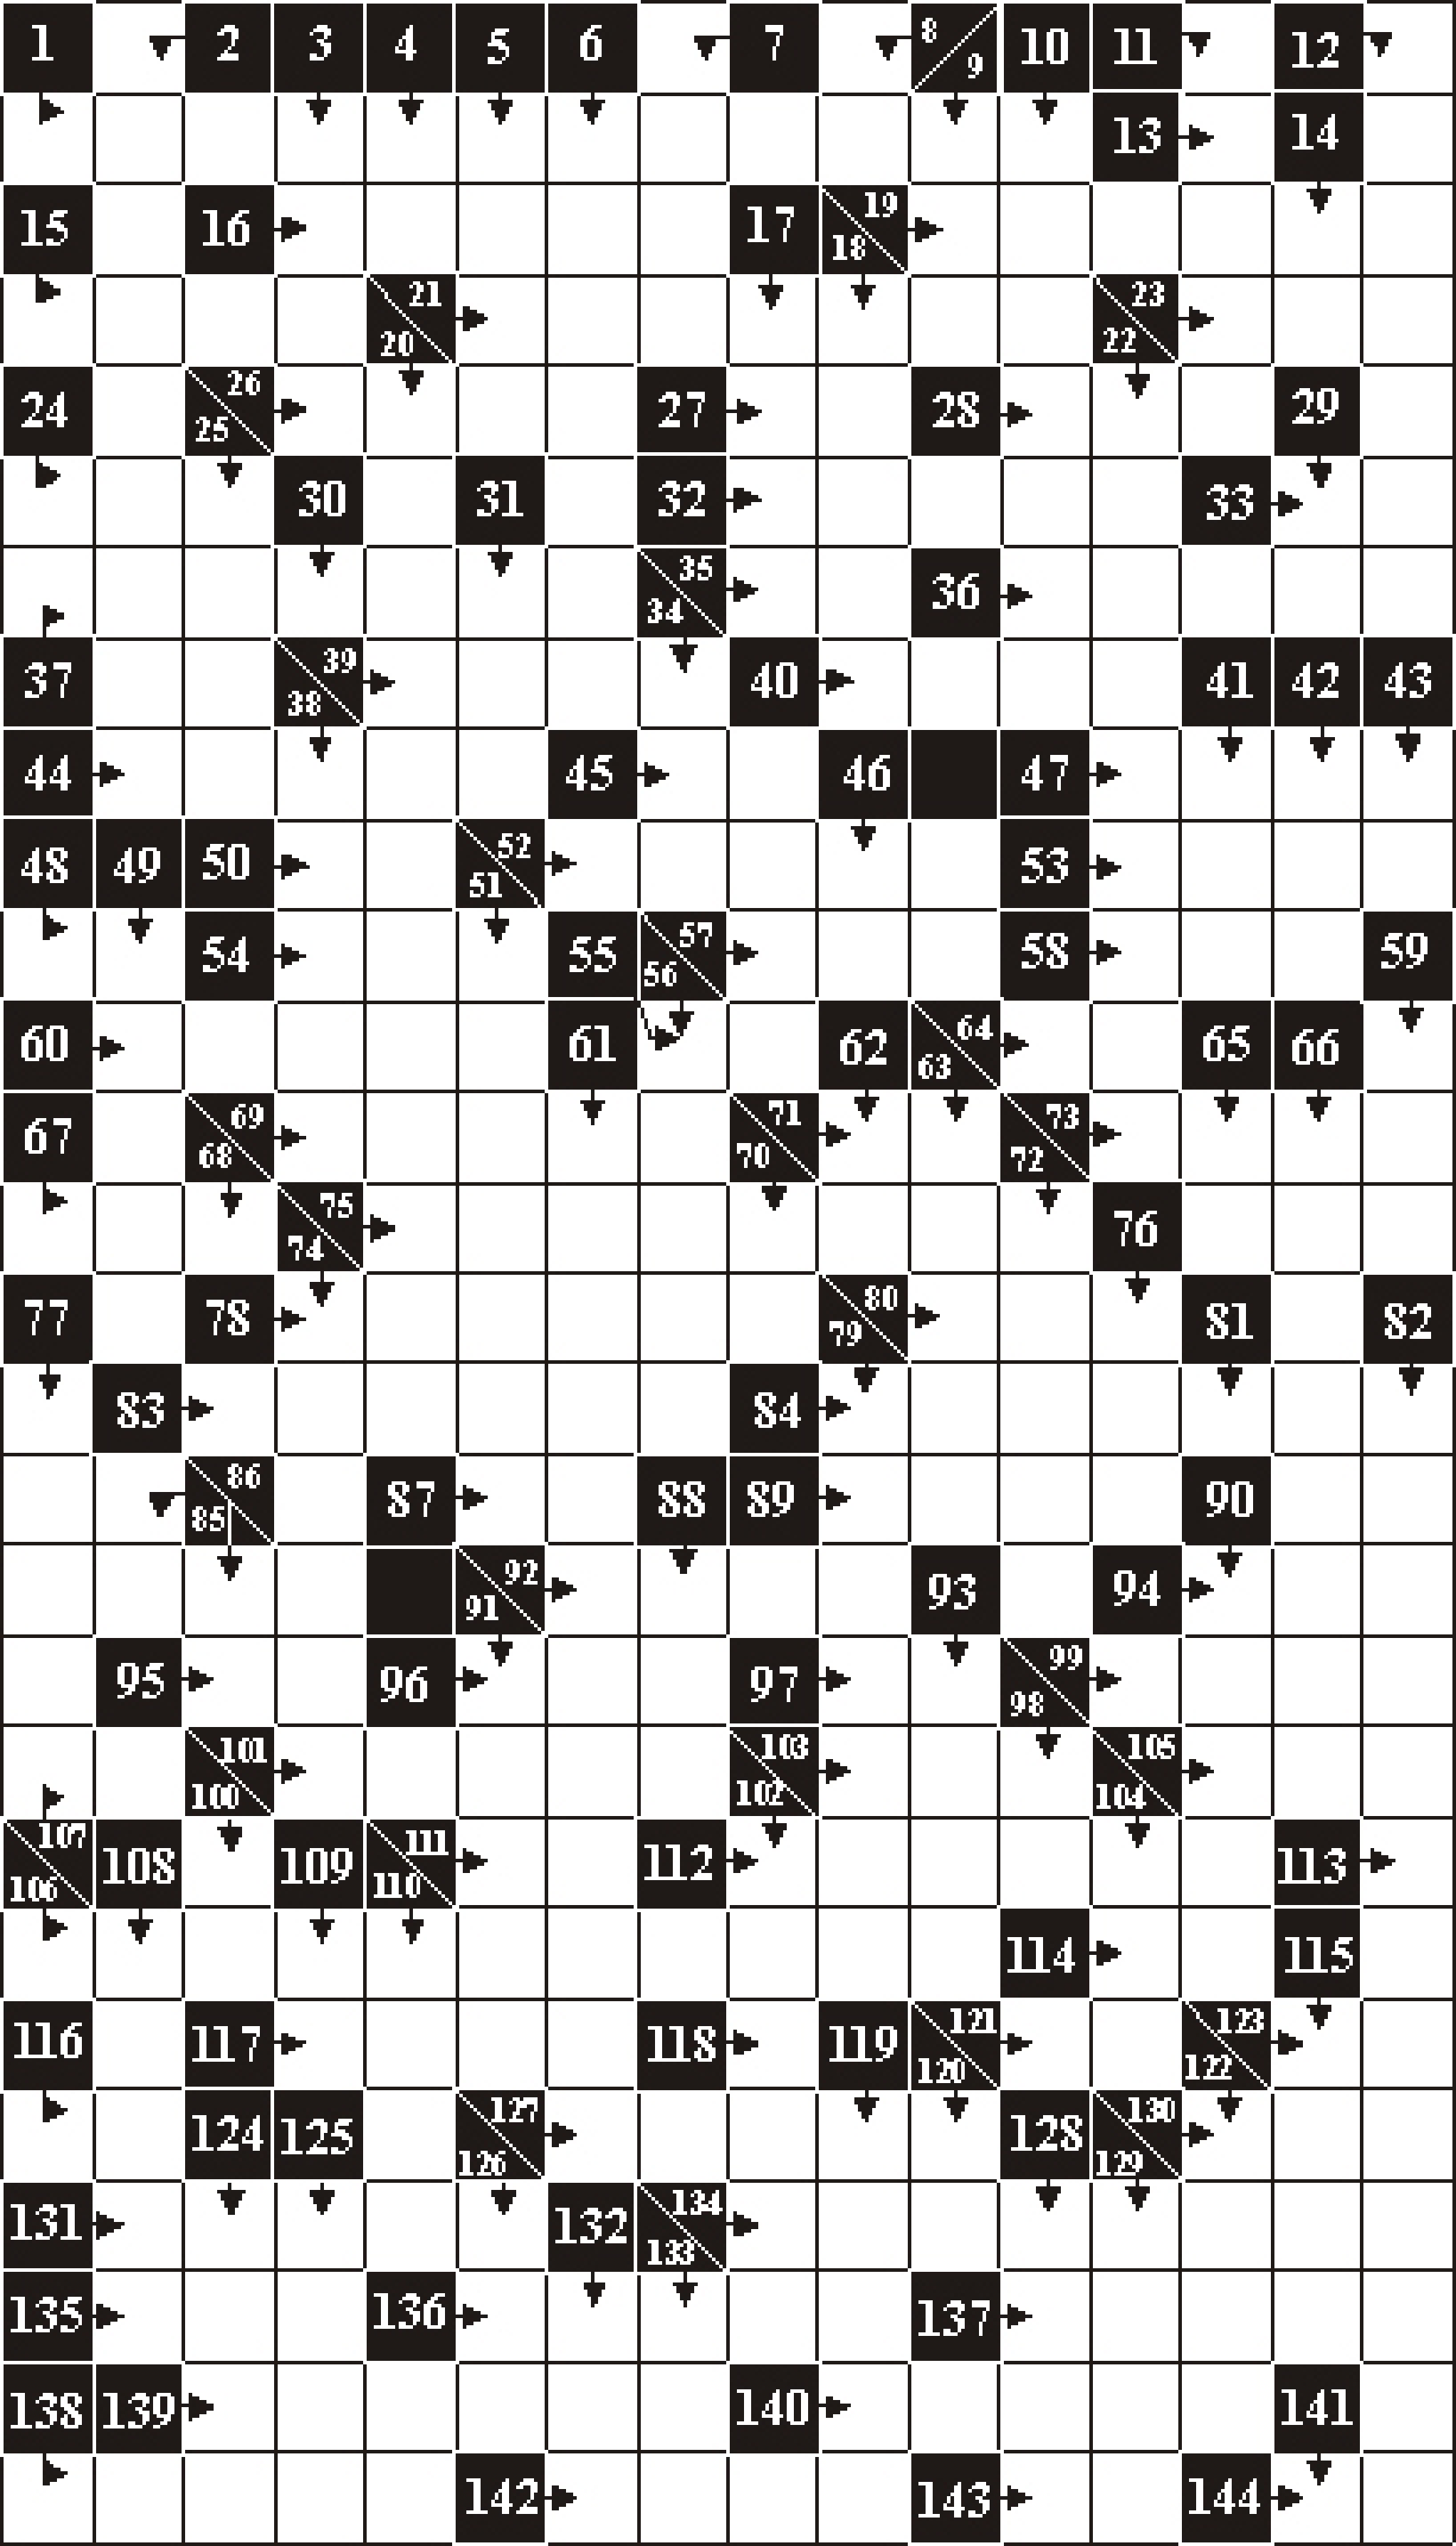
\includegraphics[height=\textheight]{res/kreuzwortraetsel_hires.png}
\end{center}
